\documentclass[aspectratio=169,professionalfonts]{beamer}

% 设置现代感清爽主题
\usetheme{Boadilla}
\usecolortheme{seahorse}

% 引入必要的宏包
\usepackage{graphicx}
\usepackage{amsmath}
\usepackage{booktabs}
\usepackage{xcolor}
\usepackage{xeCJK} % 支持中文，如果使用 pdfLaTeX 编译请换成 \usepackage{ctex}

% 隐藏导航符号，让页面更干净
\setbeamertemplate{navigation symbols}{}

% 封面信息
\title[矩阵分析与概念子空间]{矩阵的隐喻：解剖大模型概念空间与偏见}
\subtitle{线性特征提取在现代 NLP 表征中的应用}
\author[Runnel Zhang]{Runnel Zhang}
\institute[NJU]{南京大学}
\date{\today}

\begin{document}

% 1. 封面页
\begin{frame}
    \titlepage
\end{frame}

% 2. 引入与数学基础 (Setup)
\begin{frame}{理论基础：作为概念提取器的特征分析}
    \textbf{传统视角：} PCA 是一种降维压缩工具。\\
    \textbf{大模型视角（线性表征假说）：} 深度神经网络会在高维隐空间中，使用简单的线性方向来编码高级的抽象语义（如性别、时态）。
    
    \vspace{0.5cm}
    我们构建带有“性别”对立关系的词向量差值矩阵 $X \in \mathbb{R}^{n \times d}$：
    $$X_{diff} = \vec{Word}_{male} - \vec{Word}_{female}$$
    
    求解其协方差矩阵的特征分解（或直接 SVD）：
    $$\Sigma \mathbf{v}_i = \lambda_i \mathbf{v}_i \quad \text{其中} \quad \Sigma = \frac{1}{n-1} X^T X$$
    
    \textbf{物理意义：} 最大特征值对应的特征向量 $\mathbf{v}_1$，即为空间中的“性别概念方向”。
\end{frame}

% 2.5 补充：矩阵与降维核心概念辨析
\begin{frame}{概念透视：差值矩阵、特征分解与 SVD}
    为了更直观地理解上述数学操作的核心：
    \begin{itemize}
        \item \textbf{词向量差值矩阵 ($X$)}：收集“男性-女性”等配对词的差异走向。每一行代表一个“差异箭头”，记录了性别区别在不同词对中的表现。
        \item \textbf{协方差矩阵 ($\Sigma$) 与特征分解}：目的在于分析这些向量的整体分布。其最大特征值对应的\textbf{特征向量}代表“核心共识方向”（即性别主干线），而特征值大小则反映该极化方向上的统治力。
        \item \textbf{奇异值分解 (SVD)}：与特征分解殊途同归（$V$矩阵等同于协方差的特征向量），可以对原始差异矩阵一步到位提取主干方向。
        \item \textbf{解释方差占比}：衡量主成分的显著性。单方向占比若极高（如 30.40\%），说明在该空间内“性别”这一法则占据了大量的语义信息。
    \end{itemize}
\end{frame}

% 3. 实验提取与可视化 (The Extraction)
\begin{frame}{提取结果：高维空间中的线性“性别”}
    \begin{columns}
        \begin{column}{0.5\textwidth}
            \textbf{特征分析结果：}
            \begin{itemize}
                \item 提取特征向量 $\mathbf{v}_{gender}$
                \item 第一主成分解释方差占比：\textbf{30.40\%}
                \item \textit{（在 100 维稠密空间中属于极强的单向显著性信号）}
            \end{itemize}
            \vspace{0.3cm}
            \textbf{几何直觉：}
            如图所示，尽管词汇间包含了阶级、年龄等复杂差异，但在投影平面上，所有性别对立词的连线保持着较好的\textbf{平行且等距}关系。
        \end{column}
        \begin{column}{0.5\textwidth}
            \centering
            % 请确保 pca_concept_projection.png 与 tex 文件在同一目录下
            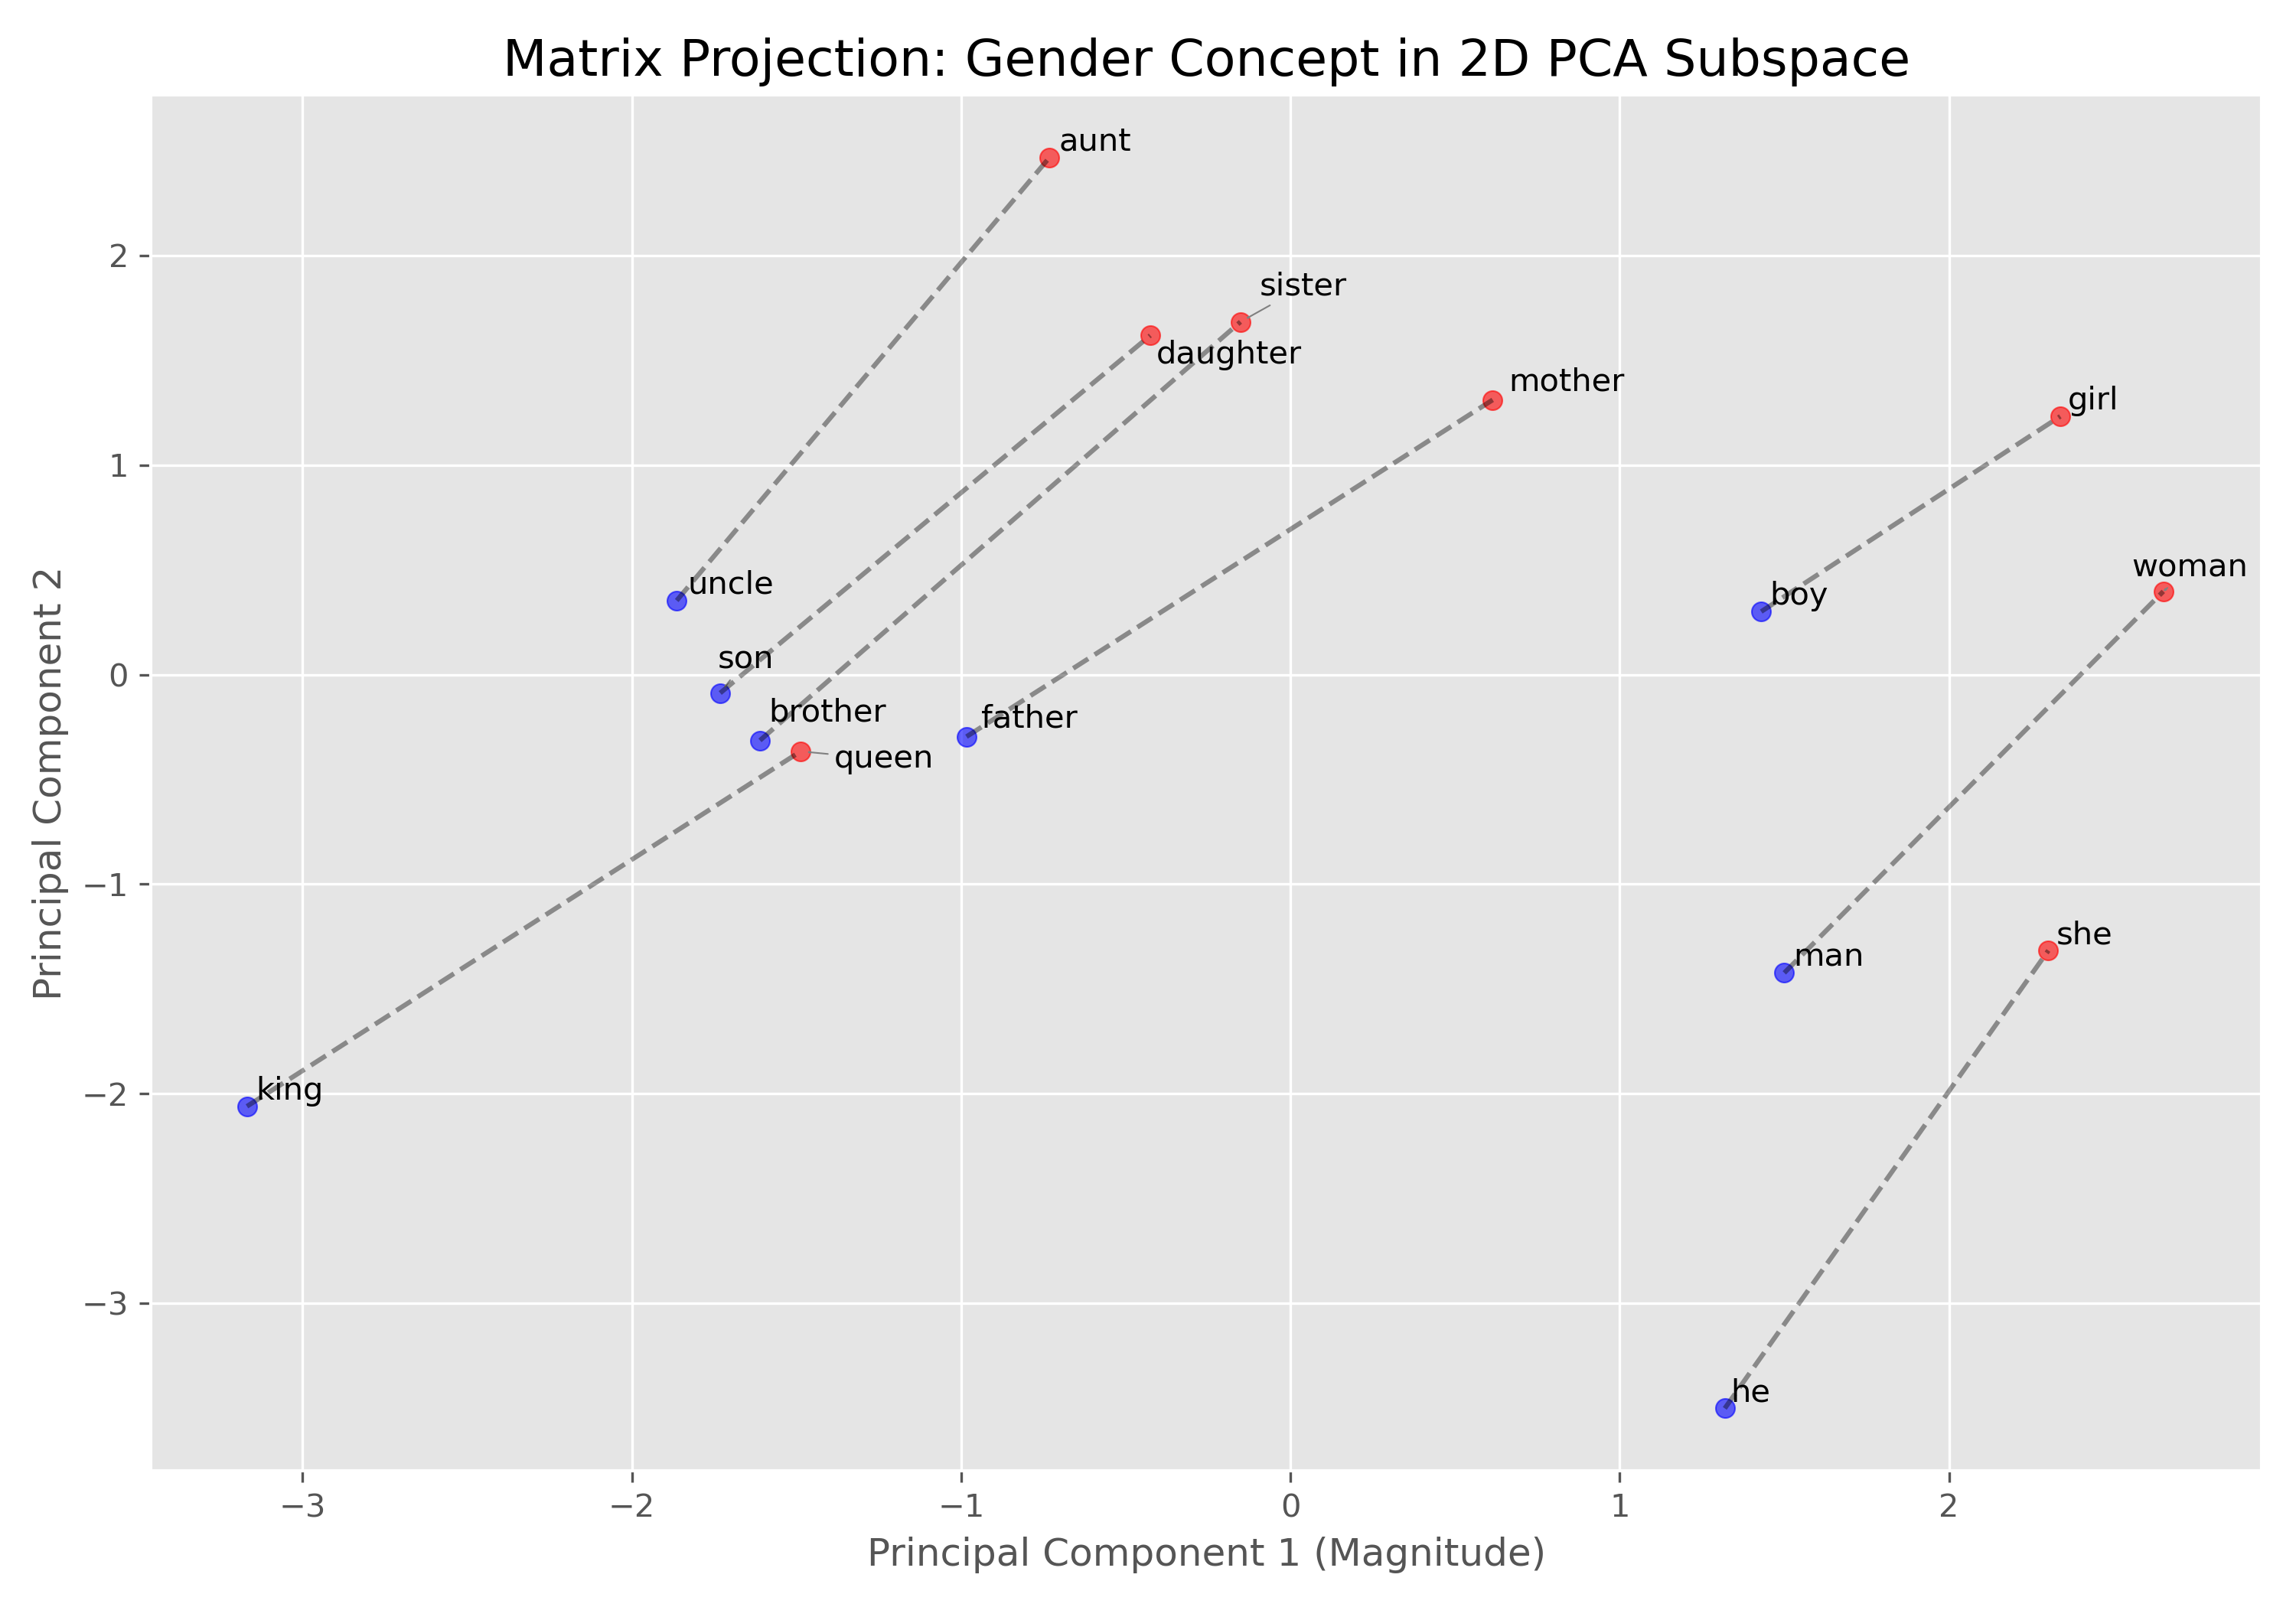
\includegraphics[width=0.9\textwidth]{pca_concept_projection.png}
        \end{column}
    \end{columns}
\end{frame}

% 4. 矩阵投影与结果分析 (The Expectation & The Twist)
\begin{frame}{矩阵投影操作：概念抹除与正交坍缩}
    \textbf{操作公式：} 使用正交投影，消除目标词汇在 $\mathbf{v}_{gender}$ 方向上的分量：
    $$\mathbf{x}_{neutral} = \mathbf{x} - (\mathbf{x}^T \mathbf{v}_{gender})\mathbf{v}_{gender}$$
    
    \vspace{0.3cm}
    \textbf{预期与实际结果：} 我们预期 King 抹去性别特征后会变成中性的 Ruler。然而真实数据表明：
    \begin{table}[]
        \centering
        \begin{tabular}{ll|ll}
        \toprule
        \multicolumn{2}{c|}{\textbf{手术前 (Original King)}} & \multicolumn{2}{c}{\textbf{手术后 (Neutralized King)}} \\ \midrule
        \textit{最近邻词} & \textit{余弦相似度} & \textit{最近邻词} & \textit{余弦相似度} \\
        prince       & 0.768               & \textbf{queen}    & \textbf{0.850} ($\uparrow$)  \\
        queen        & 0.751               & prince            & 0.777                        \\
        son          & 0.702               & \textbf{monarch}  & \textbf{0.709} (New)         \\ \bottomrule
        \end{tabular}
    \end{table}
    \textit{解释：King 和 Queen 原本是被性别维度强行拉开的。当正交投影抹平该维度后，两者坍缩到了同一个概念坐标点——纯粹的“王权”。}
\end{frame}

% 5. 纵向深挖：谱聚类的基线与跨簇迁移 (The Ultimate Twist)
\begin{frame}{谱聚类观测：流形空间中的历史偏见与跨簇迁移}
    为了更严谨地观察，我们构建了 K-NN 相似度图，并求解拉普拉斯矩阵进行谱聚类。
    
    \vspace{0.2cm}
    \textbf{1. 手术前 (Baseline) ：}
    \begin{itemize}
        \item \textbf{簇 A（统治者）：} monarch, ruler, leader, \textbf{\color{blue} king}
        \item \textbf{簇 B（象征物）：} crown, throne, palace, scepter, \textbf{\color{red} queen}
    \end{itemize}
    \textit{发现：在未经干预的原始空间中，Queen 已经被边缘化为“附属象征物”。}
    
    \vspace{0.2cm}
    \textbf{2. 手术后 (正交投影后)：}
    \begin{itemize}
        \item \textbf{簇 A（统治者）：} monarch, ruler, leader
        \item \textbf{簇 B（象征物）：} crown, throne, \dots, \textbf{\color{red} neutral\_queen}, \textbf{\color{red} neutral\_king ($\downarrow$)}
    \end{itemize}
    \textit{现象：消除性别分量后，King 发生了跨簇迁移，被归类至“象征物”簇。}
\end{frame}

% 5.5 补充：谱聚类与流形拓扑概念辨析
\begin{frame}{概念透视：谱聚类、拉普拉斯矩阵与正交投影}
    \begin{itemize}
        \item \textbf{图拉普拉斯矩阵 ($L$)}：用于刻画相似度网格结构的工具。其特征分解能够揭示图谱的连通性，天然定位出结构中最易发生分离的“断裂带”。
        \item \textbf{谱聚类 (Spectral Clustering)}：基于上述拉普拉斯矩阵，结合高维词向量的\textbf{余弦相似度}自动聚类划分圈层。
        \item \textbf{正交投影 ($x_{neutral} = x - (x^T v_{gender})v_{gender}$)}：将词汇沿着目标概念主干强行坍缩（消除影子），进而获得纯净的中立语义。
    \end{itemize}
    
    \vspace{0.3cm}
    \textbf{场景诠释（跨圈社交隐喻）：}
    \begin{itemize}
        \item \textbf{原始状态：} King 加入含有 Ruler 的“统治者俱乐部”；而 Queen 却和王冠等“附属物”混在一起。
        \item \textbf{抹除与重构：} 经过“性别特征切除手术”后，King 无法继续立足于原来的统治者圈，反而加入了 Queen 的“象征物”圈。
        \item \textbf{内核：} 这意味着原始模型中 King 与前者的相似性很可能源自共享的“男性主导特征”，一旦剥离，真实的权力身份仅仅退化成了一个符号。
    \end{itemize}
\end{frame}

\begin{frame}{K-NN 相似度图与谱聚类可视化}
    \centering
    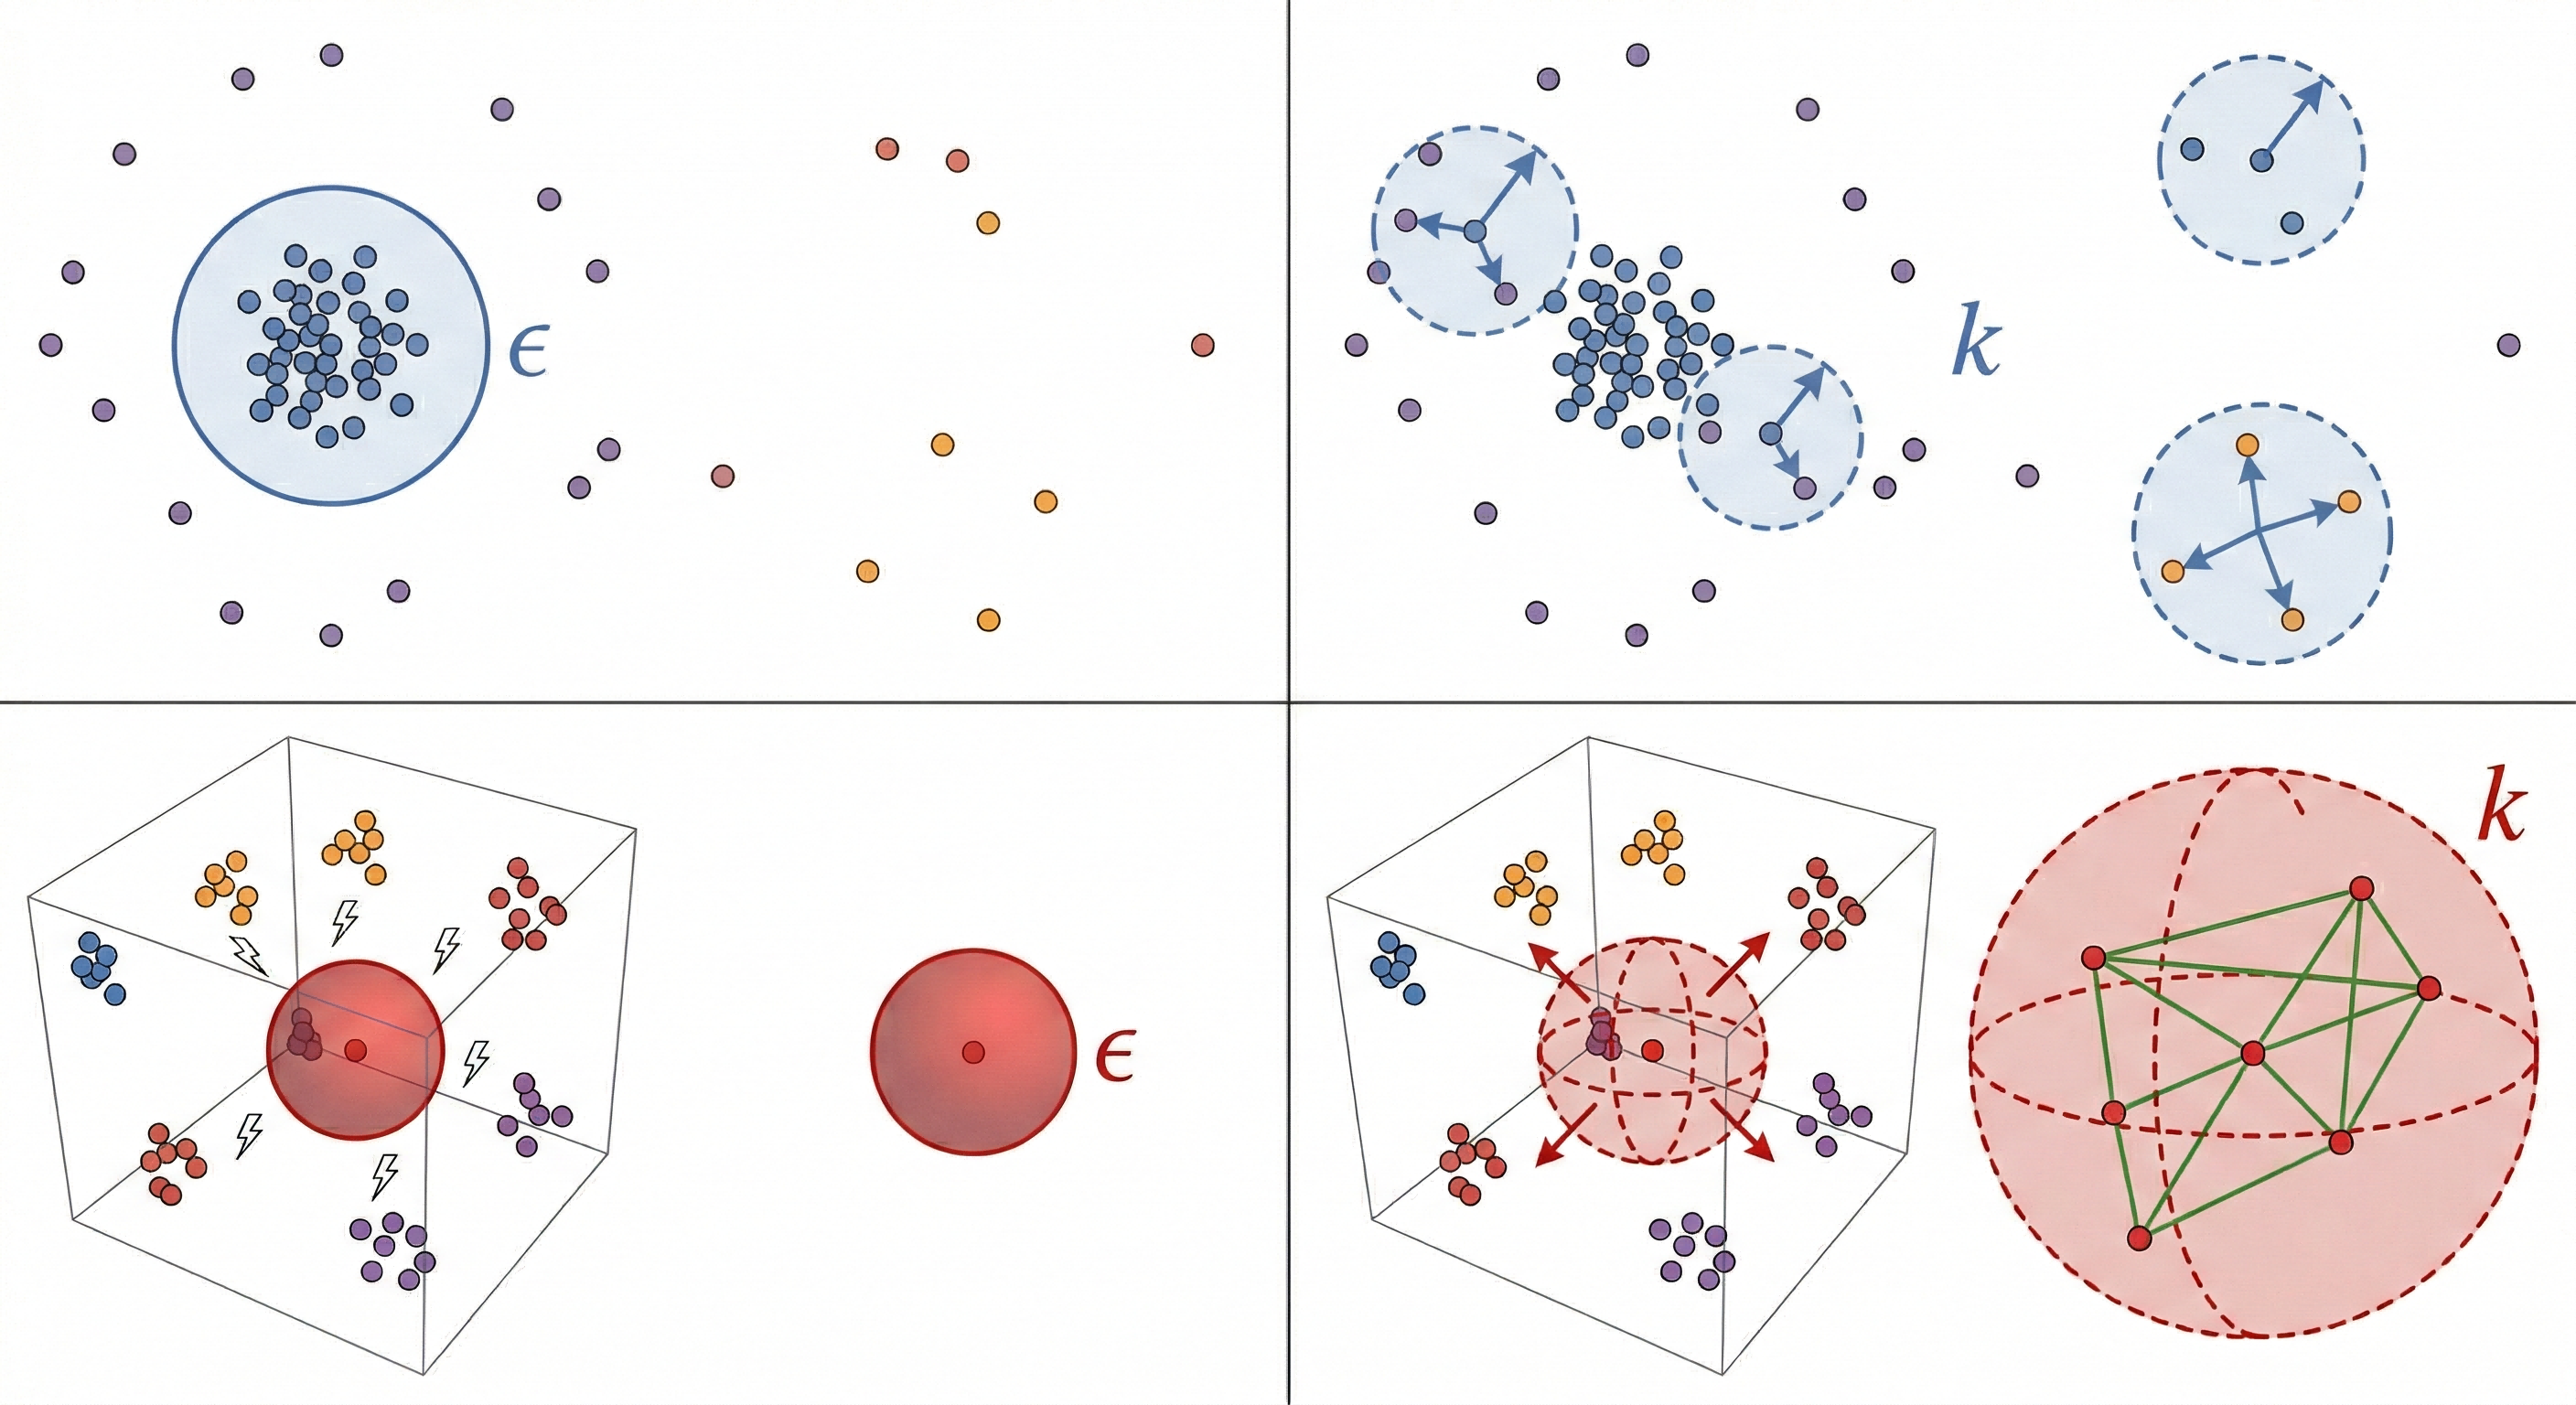
\includegraphics[width=0.8\textwidth,height=0.8\textheight,keepaspectratio]{k-nn.png}
\end{frame}

% 6. 内在机制分析 (The True Mechanism)
\begin{frame}{深入分析：语义纠缠与投影的连带影响}
    为什么 Neutral King 没有留在统治者簇，而是变成了“物品”？
    
    \vspace{0.5cm}
    \begin{itemize}
        \item \textbf{数据分布的特征耦合：} 协方差矩阵提取的 $\mathbf{v}_{gender}$ 不仅仅是生理性别，由于真实语料库的统计分布，该方向也耦合了\textbf{“主导权/主动性 (Agency)”}的方差。
        \item \textbf{正交投影的数学作用：} $\mathbf{x} - (\mathbf{x}^T \mathbf{v}_{gender})\mathbf{v}_{gender}$ 的数学操作，不仅消除了 King 的性别分量，也同时移除了与该方向共线的“主动统治”相关的语义特征。
        
    \end{itemize}
\end{frame}

% 7. 进一步探讨：逆向概率推导 (Quantitative Proof of Corpus Bias)
\begin{frame}{进一步探讨：用矩阵运算量化语料库偏见}
    为何原始空间中的 Queen 偏向物品？根据矩阵分解原理 $\vec{w}_i^T \vec{w}_k \approx \log P(k|i)$，推导出\textbf{共现概率比 (Log-Odds Ratio)}：
    $$ \vec{w}_k^T (\vec{w}_{king} - \vec{w}_{queen}) \approx \log \frac{P(k|\text{king})}{P(k|\text{queen})} $$
    
    \vspace{0.1cm}
    \textbf{预训练权重真实测算结果：}
    \begin{table}[]
        \centering
        \begin{tabular}{llc}
        \toprule
        \textbf{探针词汇 ($k$)} & \textbf{Log-Odds} & \textbf{矩阵逆推的原始语料共现概率比} \\ \midrule
        rule (统治)    & $+8.2889$ & 偏向 King \textbf{\color{red} 3979.52 倍} \\
        command (指挥) & $+5.4165$ & 偏向 King \textbf{\color{red} 225.10 倍} \\ \midrule
        beautiful (美丽)& $-5.2150$ & 偏向 Queen \textbf{\color{blue} 184.01 倍} \\
        wear (穿戴)    & $-3.6510$ & 偏向 Queen \textbf{\color{blue} 38.51 倍} \\ \bottomrule
        \end{tabular}
    \end{table}
    
    \textit{结论：矩阵运算能量化分析数据中的群体偏见分布。特征分析不仅是降维工具，也是解释模型内部表征的重要方法。}
\end{frame}

% 8. 前沿应用 (Modern Applications)
\begin{frame}{前沿应用：大模型对齐与高维知识检索}
    上述在静态词向量上的矩阵投影与干预操作，也是当前深度学习中部分研究的底层思想：
    
    \vspace{0.3cm}
    \textbf{1. 大模型表征工程 (Representation Engineering, RepE)：}
    \begin{itemize}
        \item 现代 LLM 在推理时，我们可以收集其\textbf{动态隐藏层激活矩阵 (Hidden States)}。
        \item 利用 PCA 提取出代表“诚实 (Truthfulness)”或“安全 (Safety)”的特征向量 $\mathbf{v}_{concept}$。
        \item 推理时直接执行向量干预 $\mathbf{h}_{new} = \mathbf{h} \pm \alpha \mathbf{v}_{concept}$，\textbf{无需微调即可在一定程度上影响模型输出行为或对齐价值观。}
    \end{itemize}
    
    \vspace{0.2cm}
    \textbf{2. 检索增强生成 (RAG) 中的拓扑切分：}
    \begin{itemize}
        \item 在构建面向垂直领域（如 AI4Math、AI4Sci）的复杂知识库时，海量文档的稠密向量往往会产生严重的语义纠缠。
        \item 利用\textbf{谱聚类}与图拉普拉斯特征分析，可以在高维流形上对 Document Embeddings 进行严谨的拓扑切分，构建层次化检索树，大幅降低 RAG 的幻觉与检索噪声。
    \end{itemize}
\end{frame}
% 9. 总结
\begin{frame}
    \begin{center}
        \Huge \textbf{Thanks.}
    \end{center}
\end{frame}

\end{document}